% Para documento texto corto
%\documentclass[paper=letter,oneside,fontsize=12pt, parskip=full]{article}
\documentclass[paper=letter,oneside,fontsize=11pt, parskip=full]{scrartcl}
%\documentclass{amsart}
%\documentclass[paper=letter,oneside,fontsize=12pt]{scrartcl}

% Establece dimensiones de los margenes
% \usepackage[inner=1.5cm,outer=3cm,top=2cm,bottom=4cm,
% bindingoffset=5mm]{geometry}
\usepackage[left=3cm,right=3cm,top=3cm,bottom=3cm,
bindingoffset=0cm, footskip=0.5cm, headheight=2cm]{geometry}

% Elimina sangrias y aumenta espacio entre parrafos
\usepackage{parskip}

% Permite cambiar margenes derecho e izquierdo
% de secciones de texto con el entorno
% adjustwidth
\usepackage{changepage}

% Permite establecer el espaciado entre lineas
\usepackage{setspace}

% Permite ingresar caracteres acentuados y especiales 
% sin necesidad de emplear comando
% utf8 codificacion de entrada Unicode (mas simbolos que ASCII)
\usepackage[utf8]{inputenc}

% Formato direccione URL
% \usepackage{hyperref}

% T1 encoding for European, English, American text
\usepackage[T1]{fontenc}
% Fuente escalable
\usepackage{lmodern}

% Reemplazo para fuente Arial
% \usepackage{helvet}
% Usa la fuente sans-serif por defecto
% \renewcommand{\familydefault}{\sfdefault}

% Carga babel, idioma ingles
\usepackage[english, spanish]{babel}

% Mejor jsutificacion, tipografia alta calidad.
\usepackage{microtype}
% Para unir columnas y filas en tablas
\usepackage{array}

% Agrega comandos extra al comando tabular
% \toprule, \midrule, \bottomrule
\usepackage{booktabs}
% Tablas con ancho establecido por usuario
\usepackage{tabularx}
% Para posicionamiento preciso de tablas dentro del texto
\usepackage{float}

% Unir filas en tablas
\usepackage{multirow}

% Permite controlar colores de tablas
\usepackage{xcolor, colortbl}

% Encabezados personalizados
\usepackage{fancyhdr}
\usepackage{graphicx}

% Permite obtener el numero de la ultima pagina
\usepackage{lastpage}

% Paquetes para figuras
% Paquete caption para titulos figuras
% Paquete subcaption para subfiguras
\usepackage{caption}
\usepackage{subcaption}

% Espaciado inteligente
\usepackage{xspace} 

% Para formato de codigo fuente
\usepackage{xcolor}
\usepackage{listings}
% Etiquetas de listandos codigo en españoñ
\renewcommand\lstlistingname{Listado}

\lstset{basicstyle=\ttfamily,
	showstringspaces=false,
	commentstyle=\color{red},
	keywordstyle=\color{blue}}

% Cabeceras
\pagestyle{fancy}
% Borra cabecera y pie actuales
\fancyhead{}
% Cintillo cabecera
%\chead{
%	\includegraphics[width=150mm]{Imagenes/Cabecera.png}
%}
%\fancyhead[L]{\includegraphics[width=0.3\textwidth]{Imagenes/cabecera.pdf}}
%\fancyfoot[C]{ 
%	\begin{tabularx}{\textwidth}{|m{2.0cm}|X|m{2.5cm}|m{2.0cm}|}
%		\hline			
%			\centering
%			\includegraphics[height=0.8cm]{Imagenes/pie-izq.pdf} &			
%			\centering
%			Confidencial &
%			\centering
%			\includegraphics[height=0.8cm]{Imagenes/pie-der.pdf}  &			
%			\thepage~/~\pageref{LastPage} \\
%		\hline 
%	\end{tabularx}	 
%}

% Comando para formatear y justificar parrafos de código y 
% comandos de shell
% \newcommand{\code}[1]{
%	\begin{adjustwidth}{1.5cm}{0.0cm}
%		\ttfamily
%		#1
%	\end{adjustwidth}}	

% Entorno para formato de secciones de codigo
\newenvironment{code}
	{\begin{adjustwidth}{1.5cm}{0.0cm}\ttfamily}
	{\end{adjustwidth}}

% Entorno para formato de secciones de enlaces
\newenvironment{link}
	{\ttfamily}{}	
	
\definecolor{colorfa}{rgb}{0.3569,0.608,0.8353}
\definecolor{colorfb}{rgb}{0.4392,0.678,0.2784}
\definecolor{colorfc}{rgb}{1.0000,0.361,0.0000}
\definecolor{colorsem}{rgb}{0.1804,0.455,0.7098}
\definecolor{colorfd}{rgb}{0.9294,0.490,0.1922}
\definecolor{colorfe}{rgb}{0.2667,0.329,0.4157}

\newcommand{\fa}{\cellcolor{colorfa}}
\newcommand{\fb}{\cellcolor{colorfb}}
\newcommand{\fc}{\cellcolor{colorfc}}
\newcommand{\sem}{\cellcolor{colorsem}}
\newcommand{\fd}{\cellcolor{colorfd}}
\newcommand{\fe}{\cellcolor{colorfe}}

% Numeracion de paginas
% numeros arabigos
\pagenumbering{arabic}

	\begin{document}
		
		%\title{Informe de Avance de Pasantía}
		%\author{Jose Arias}
		%\address{correo@josearias.com.ve}
		%\date{Septiembre, 2017}
		
		%\maketitle
			
		\begin{titlepage}
		
		\begin{center}		
			
			%\vspace{10cm}
			% 12 puntos = fuente large
			\begin{large}							
				\bfseries
				\uppercase{Universidad Central de Venezuela} \\			
				\uppercase{Facultad de Ingeniería} \\							
				\uppercase{Escuela de Ingeniería Eléctrica} \\
        		\uppercase{Departamento de Electrónica, Computación y Control} \\
        		\uppercase{Anteproyecto de Trabajo Especial de Grado}          	
			\end{large}			
		
			\vfill
			
			\begin{large}
				\bfseries
				\uppercase{Informe de Avance de Pasantía}
			\end{large}
		
			\vspace{2mm}
			
			% 16 puntos = fuente Large de 14 puntos			
			\begin{Large}
				\begin{spacing}{1.2}
					\bfseries				
		      		\uppercase{Diseño de un equipo electrónico controlador de interruptores y atenuadores empleado en la medición de la figura de ruido en dispositivos de radio frecuencia}	
		      	\end{spacing}
			\end{Large}					
			
			\vfill
			
			\begin{flushright}
				Br. Arias Bustamante, Jose A. \\
				C.I. 14.66.744.
			\end{flushright}
		
			\vfill
			
			\begin{center}
				Caracas, septiembre 1017.
			\end{center}
		
		\end{center}
	
	\end{titlepage}
	
	\clearpage
	
	\tableofcontents
		
	\section{Introducción}
		Describe el proceso de instalación adaptador USB/GPIB Agilent 82357B, la instalación y construcción de la librería c de soporte (\texttt{linux-gpib}) a partir del código fuente y la obtención y carga del firmware para el adaptador.
		
	\section{Descripción del Proyecto}
	
	En la figura \ref{Fig:SistemaMedicionFiguraRuido} se muestra un sistema propuesto por Agilent Technologies para medición de la figura de ruido en dispositivos de radio frecuencia y de microondas. Este sistema esta conformado por tres instrumentos fundamentales.
	
	\begin{table}[h!]
		\begin{tabular}{p{3cm}l}
			\begin{minipage}{3cm}
				\includegraphics[width=3cm]{Imagenes/N8975A.pdf}
			\end{minipage} &
			Analizador de figura de ruido (NFA) N8975A \\

			\begin{minipage}{3cm}
				\includegraphics[width=3cm]{Imagenes/N2002A.pdf}
			\end{minipage} &
			Equipo para pruebas con fuente de ruido N2002A \\
			
			\begin{minipage}{3cm}
				\includegraphics[width=3cm]{Imagenes/11713A.pdf}
			\end{minipage} &			
			Controlador electrónico de interruptores y atenuadores, serie 11713 
		\end{tabular}
	\end{table}

	De los tres equipos listados, el Cendit dispone solo dos de ellos: el analizador de figura de ruido N8975A y el equipo para pruebas con fuente de ruido N2002A. Para que la institución pueda colocar en servicio el SMFR, requiere del controlador electrónico de atenuadores de la serie 11713 de Keysight Technologies. Por motivos presupuestarios, este equipo no ha podido ser adquirido.
	
	Para suplir esta carencia, el Cendit requiere el diseño de un equipo electrónico que pueda suplir la funcionalidad de los equipos de la serie 11713 dentro del sistema. El diseño de este dispositivo es el tema del TEG del cual este documento es un informe de avance de pasantia.
	
	\begin{figure}[h!]
		\begin{center}
			\includegraphics[width=17cm]{Imagenes/DiagramaBloquesSistema.pdf}
			\caption{Esquema de sistema para medición de figura de ruido}
			\label{Fig:SistemaMediciónFiguraRuido}
		\end{center}
	\end{figure}			
	
	
	\begin{figure}[!h]
		\begin{center}
			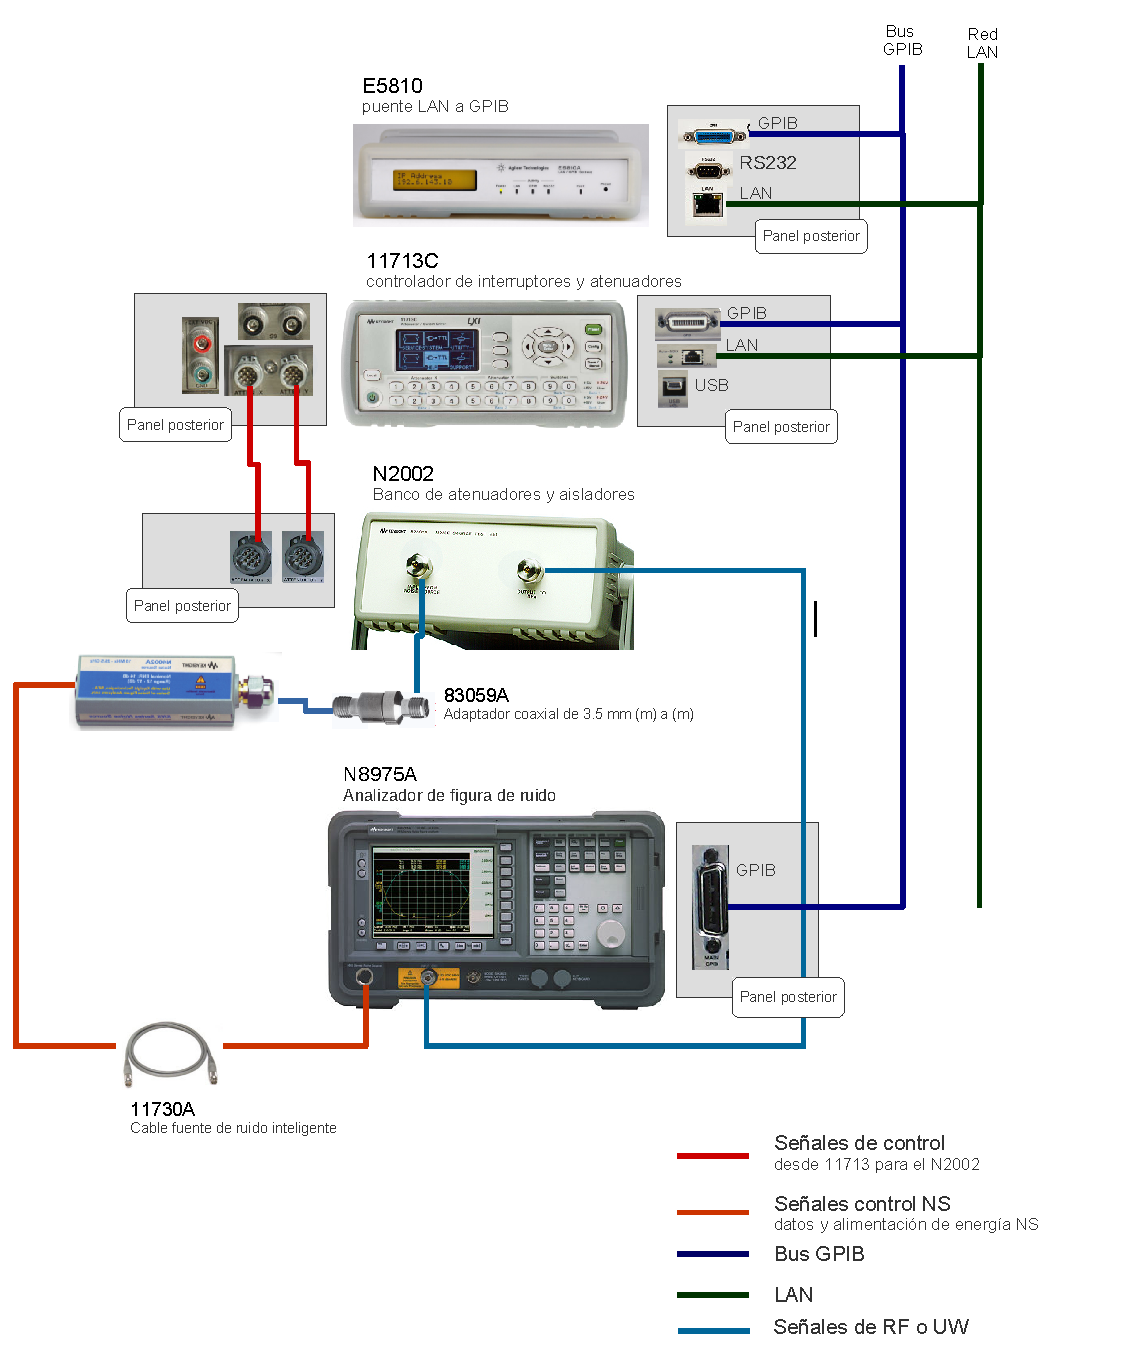
\includegraphics[height=6cm]{Imagenes/SistemaMedicionFiguraRuido.pdf}
			\caption{Sistema para medición de figura de ruido}
			\label{Fig:SistemaMedicionFiguraRuido}
		\end{center}	
	\end{figure}	

	\begin{figure}[h!]
		\begin{center}
			\includegraphics[width=18cm]{Imagenes/DiagramaBloquesHardware2.pdf}
			\caption{Diagrama de Bloques Hardware}
			\label{Fig:Diagrama de Bloques de Hardware}
		\end{center}
	\end{figure}




	\subsection{Metodología Inicial}
	
	\subsection{Cronograma de Actividades}
	
	\begin{table}[!h]
		\centering
		\arrayrulecolor{gray}
		\setlength{\extrarowheight}{4pt}		
		\resizebox{\textwidth}{!}{
		\begin{tabular}{|c|l|l|l|l|l|l|l|l|l|l|l|l|l|l|l|l|l|l|l|l|l|l|l|l|l|l|l|l|}
			\hline 			
			\textbf{Semanas} & 1 & 2 & 3 & 4 & 5 & 6 & 7 & 8 & 9 & 10 & 11 & 12 & 13 & 14 & 15 & 16 & 17 & 18 & 19 & 20 & 21 & 22 & 23 & 24 & 25 & 26 & 27 & 28 \\
			\hline
			\textbf{Fase 1}
			& \fa & \fa & \fa & \fa & \fa & \fa & & & & & & & & & & & & & & & & & & & & & & \\			
			\hline			
			\textbf{Fase 2} & & & & & & & \fb & \fb & \fb & \fb & \fb & \fb & \fb & \fb & \fb & \fb & \fb & & & & & & & & & & & \\
			\hline
			\textbf{Fase 3} & & & & & & & & & & & & & & & & & & \fc & \fc & \fc & \fc & \fc & & & & & & \\	
			\hline		
			\textbf{Seminario} & & & & & & & & & & & & & & \sem & & & & & & & & & & & & & & \\
			\hline
			\textbf{Fase 4} & & & & & & & & & & & & & & & & & & & & & & & \fd & \fd & \fd & \fd &  & \\
			\hline
			\textbf{Fase 5} & & & & & & & & & & & & & & & & & & & & & & & & & & & \fe & \fe \\
			\hline
		\end{tabular}
		}
	\end{table}
	

	\begin{table}[h!]
		\begin{tabular}{rp{13cm}}
			\textbf{Fase 1} & Preparación e investigación. Dedicada a investigar el funcionamiento de cada uno de los equipos que integran el sistema de medición de figura de ruido. La recopilación y lectura de la documentación de estos equipos que ofrecen las empresas Agilent y Keysight y a través de ensayos sobre el sistema se obtendrá un entendimiento del funcionamiento del mismo. La información obtenida se plasmará en un informe descriptivo del SMFR. \\			
			\textbf{Fase 2} & Diseño de hardware. Comienza con la formulación de un concepto para un equipo que permita suplir la funcionalidad de un equipo de la serie Keysight 11713. Por medio de un proceso iterativo que implica el diseño de hardware, de firmware y mecánico se logrará la documentación de diseño, que permita construir el hardware en la siguiente fase.	\\		
			\textbf{Fase 3} & Implementación del hardware. Se construirá el hardware diseñado y se verificará su desempeño dentro del SMFR. Esta fase implica la depuración firmware y software además de verificar que el hardware cumpla los objetivos de diseño. \\
			\textbf{Fase 4} & Preparación de manuales. Se producirá un manual de usuario para el equipo implementado, que contendrá instrucciones para instalación, operación y resolución de fallas. \\
			\textbf{Fase 5} & Preparación de documentos Cierra el proyecto con la preparación de un informe de pasantía para el Cendit. También se elabora el tomo parra TEG, a presentar en la Escuela de Ingeniería Eléctrica de la UCV.
		\end{tabular}
	\end{table}

	\section{Actividades Realizadas}
	
	\subsection{Preparación inicial}
	\subsection{Documentación bibliográfica acerca del SMFR}
	\subsection{Investigación y recopilación de software asociado al SFRM}
	\subsection{Diseño de hardware}
	\subsection{Diseño de software}
	\subsection{Documento de captura de requerimientos de software}
	\subsection{Búsqueda, selección y pedido de componentes electrónicos}
	
	\subsection{Elaboración de intrucciones de trabajo}

	

	

\end{document}